%% ICAIF '26 submission — anonymous review version.
%%
%% Compile on Overleaf with the ACM template (acmart). Locally:
%%     latexmk -pdf icaif26.tex
%%
%% Remove the `anonymous,review` options for the camera-ready and fill in the
%% author block. Requires: refs.bib and figures/ alongside this file.
%%
%% PAGE BUDGET. ICAIF allows 8 pages INCLUDING figures and references;
%% over-length papers are rejected without review. This source was written to a
%% ~3,800-word body against that budget but has NOT been compiled — check the
%% page count first and cut from the marked \ICAIFcut regions if over.

\documentclass[sigconf,anonymous,review]{acmart}

\AtBeginDocument{%
  \providecommand\BibTeX{{\normalfont B\kern-0.5em{\scshape i\kern-0.25em b}\kern-0.8em\TeX}}}

\setcopyright{acmlicensed}
\acmConference[ICAIF '26]{ACM International Conference on AI in Finance}{November 14--17, 2026}{Milan, Italy}

\usepackage{booktabs}
\usepackage{amsmath}

% Marks a region that can be cut first if the page count runs over.
\newcommand{\ICAIFcut}{}

\begin{document}

\title{Regime Effects Are Turnover Effects}
\subtitle{Matched Controls for Conditional Portfolio Optimization}

\author{Anonymous Author(s)}

\begin{abstract}
Conditioning portfolio allocation on an inferred market regime is widely reported
to improve risk-adjusted performance, particularly net of transaction costs. We
show that in a cardinality-constrained US equity setting the measured effect is
explained entirely by \emph{turnover}: a persistent state estimate produces
persistent allocations, so the conditioned strategy trades less --- and trading
less is what pays.

We evaluate 32 arms on CRSP daily data (2011--2024, 168 monthly rebalances, 30
matched seeds per arm, four transaction-cost levels), injecting a three-state
hidden Markov signal at each of the three points where it can act on a
mean--variance decision: the optimizer's preference parameters, its covariance
estimate, and its expected-return vector. All three appear to work, gaining
$+0.113$, $+0.388$ and $+0.294$ Sharpe at 150\,bps per trade. Across 27
comparable arms, net-of-cost performance is ordered by realized turnover alone
(Spearman $\rho = -0.95$, $p = 2.1\times10^{-14}$); gross of costs the same
correlation is insignificant.

The decisive comparison is a control we solve rather than assume: an
unconditional arm whose turnover penalty is found by bisection until it trades
exactly as much as the treatment. Against it the effect is $-0.069$, $-0.034$ and
$-0.047$ Sharpe --- negative at every injection point and every cost level.
Permutation controls beat their treatments, untimed parameterizations beat timed
ones, and perfect foreknowledge of the state is worth $+0.010$.

We also bound what such studies can resolve: re-running one arm under a different
random seed, with identical data and configuration, moves realized Sharpe by
$0.233$ and fourteen-year terminal wealth by $1.85\times$. \textbf{Any conditional
strategy reported to beat an unconditional baseline net of costs should be
measured against a turnover-matched control.}
\end{abstract}

\begin{CCSXML}
<ccs2012>
<concept><concept_id>10010147.10010257</concept_id><concept_desc>Computing methodologies~Machine learning</concept_desc><concept_significance>500</concept_significance></concept>
<concept><concept_id>10010405.10010444.10010449</concept_id><concept_desc>Applied computing~Economics</concept_desc><concept_significance>500</concept_significance></concept>
<concept><concept_id>10002950.10003648.10003688</concept_id><concept_desc>Mathematics of computing~Probability and statistics</concept_desc><concept_significance>300</concept_significance></concept>
</ccs2012>
\end{CCSXML}

\ccsdesc[500]{Computing methodologies~Machine learning}
\ccsdesc[500]{Applied computing~Economics}
\ccsdesc[300]{Mathematics of computing~Probability and statistics}

\keywords{portfolio optimization, regime switching, transaction costs, evaluation
methodology, matched controls, reproducibility, hidden Markov models}

\maketitle

%% =====================================================================
\section{Introduction}

Mean--variance selection~\cite{Markowitz1952} becomes a mixed-integer quadratic
program once practical constraints are imposed: a bound on the number of holdings,
box constraints on each position, a penalty on trading. A large applied literature
solves the constrained problem with population
metaheuristics~\cite{Chang2000,Ertenlice2018,Kalayci2019}, and a parallel
literature conditions the resulting allocation on an inferred market
state~\cite{AngBekaert2002,GuidolinTimmermann2007,Kritzman2012,Nystrup2015}.
Reported results in the second literature are generally favorable, particularly
net of transaction costs.

This paper argues that those results are an artifact with a specific, testable
form.

\paragraph{The confound.} A regime-conditioned strategy inherits the persistence
of its state estimate. A posterior that remains in one state for months produces
allocations that remain in one place for months, so the conditioned strategy
\emph{trades less} than its unconditional counterpart --- for reasons unrelated to
whether it has identified anything about the market. When performance is reported
net of costs, turnover and conditioning are confounded by construction.

\paragraph{The control.} The obvious objection is that turnover reduction
\emph{is} the mechanism working: a regime model that recognizes it should sit still
has earned its keep. We answer that objection with a control designed for it. For
each treatment we solve, by bisection on the turnover penalty $\lambda_t$, for an
\emph{unconditional} arm that trades exactly as much as the treatment. Same
optimizer, same constraints, same seeds, same realized turnover, no regime model.
If the signal contributes anything beyond the trading volume it induces, the
treatment must beat this control. It does not.

\paragraph{Exhaustiveness.} A negative result about one injection point invites the
reply that the signal was injected in the wrong place. We therefore enumerate: a
state signal can act on a mean--variance decision by changing what the optimizer
\emph{wants} (preference parameters), what it \emph{believes} about risk
($\boldsymbol{\Sigma}$), or what it \emph{expects} about return
($\boldsymbol{\mu}$). Figure~\ref{fig:injection} is the taxonomy. We build all
three, hold the solver identical across them, and give each its own permutation
control, lookahead oracle, and turnover-matched control.

Every cell of that design returns the same answer. What we contribute is therefore
not a strategy but an apparatus for deciding whether one works, together with a
measure of how much of any such decision is noise.

\paragraph{Contributions.}
\begin{enumerate}
\item A \textbf{turnover-matched control} for conditional allocation, solved by
bisection against a treatment's realized trading, and the demonstration that it
eliminates the effect at every injection point.
\item A \textbf{complete negative result}: conditioning of preferences, beliefs and
expected returns, each against three independent controls, is null or negative.
\item A \textbf{quantified noise floor} for a population metaheuristic on this
problem, measured against the effect sizes the surrounding literature reports.
\item A reproducible harness with a machine-checked lookahead proof, permutation
controls preserving marginals and dwell times, oracle bounds, and reproduction
verified by re-execution. It caught three silent confounds in this study.
\end{enumerate}

We are explicit about what is not new. The optimizer is a firefly--particle-swarm
hybrid in the manner of~\cite{Aydilek2018} applied to the problem
of~\cite{Bacanin2014}; it is the instrument, not a contribution. That seed variance
can swamp published effects is due to~\cite{Henderson2018} in reinforcement
learning and to~\cite{GilliSchumann2011} in portfolio heuristics; our contribution
is its magnitude in a setting that has not been audited.

%% =====================================================================
\section{Related Work}

\paragraph{Constrained selection.} \citet{Chang2000} gave the seminal metaheuristic
treatment and established the benchmark instances the literature reuses;
\citet{WoodsideOriakhi2011} revisited them with improved population heuristics.
Swarm intelligence is now the dominant family~\cite{Ertenlice2018}, with particle
swarm optimization most frequently applied~\cite{Cura2009,Zhu2011} and with
documented failure modes~\cite{Deng2012}. The firefly
algorithm~\cite{Yang2008,Fister2013} replaces attraction to a single global best
with distance-decaying pairwise attraction and has been applied to this exact
problem~\cite{Bacanin2014}. Across this literature --- 175 papers
in~\cite{Kalayci2019} --- results are reported as a single objective value or a
single backtest; seed-to-seed dispersion of the returned decision is rarely
reported.

\paragraph{Conditional allocation.} \citet{AngBekaert2002} solve dynamic allocation
under regime-switching correlations; \citet{GuidolinTimmermann2007} identify four
states governing joint stock--bond returns; \citet{Kritzman2012} report that a
dynamic regime-based process outperforms static allocation in backtests,
``especially for investors who seek to avoid large losses'';
\citet{Nystrup2015} compare regime-based against static allocation directly. The
injection point differs across authors and is rarely compared within one design,
and turnover is confounded with conditioning whenever results are reported net of
costs. We are not aware of published work in this literature that separates them
with a control matched on turnover.

\paragraph{Solver reliability.} \citet{GilliSchumann2011} address the stochasticity
of heuristic solutions in portfolio optimization directly, arguing that the
randomness of the returned solution can be made practically negligible and that the
in-sample/out-of-sample relationship is non-monotonic. We build on both. At the
budgets the applied literature uses, the residual randomness is not negligible: it
exceeds effect sizes that literature reports. The methodological template
is~\citet{Henderson2018}. This is distinct from the backtest-overfitting
literature~\cite{Bailey2014,Bailey2017}, which audits \emph{selection across}
strategies; we audit \emph{solver variance within} one strategy. That optimizing
harder against noisy inputs can degrade decisions is long
established~\cite{Michaud1989,DeMiguel2009,BottouBousquet2007}.

%% =====================================================================
\section{Problem Setting}

At each rebalance the optimizer receives $\boldsymbol{\mu}$, $\boldsymbol{\Sigma}$
and the previous holdings $\mathbf{w}_{\mathrm{prev}}$, and maximizes
\begin{equation}
R(\mathbf{w}) = \boldsymbol{\mu}^\top \mathbf{w}
- \lambda_v \sqrt{\mathbf{w}^\top \boldsymbol{\Sigma}\mathbf{w}}
- \lambda_t \cdot \mathrm{TO}(\mathbf{w}, \mathbf{w}_{\mathrm{prev}})
\end{equation}
subject to $\sum_i w_i = 1$, $l_i \le w_i \le u_i$ and
$|\{i : w_i > 0\}| \le K$, where
$\mathrm{TO}(\mathbf{w},\mathbf{w}_{\mathrm{prev}}) =
\tfrac{1}{2}\lVert \mathbf{w}-\mathbf{w}_{\mathrm{prev}}\rVert_1$
is \textbf{one-way} turnover. Costs are charged per trade on traded notional, the
standard quotation; rotating a position generates both a sale and a purchase, so
the realized drag is $2c\cdot\mathrm{TO}$ for a per-trade rate $c$. We report cost
levels per trade throughout and state the factor explicitly, because the product of
these two quantities is this paper's subject.

Constraints are handled by projection rather than penalty: every candidate is
repaired onto the feasible set before evaluation, so the search never leaves it.
The search is a firefly--particle-swarm hybrid; each particle's move is a convex
combination, with constant blend $\phi = 0.5$, of a firefly step toward the
brightness-weighted centroid of brighter peers and a PSO step toward personal and
global bests, run at 30 particles for 60 iterations.

\textbf{The solver is the instrument, not the contribution.} It is used because the
constraint set is non-convex and gradient-free search handles it natively.
Section~\ref{sec:conviction} reports that removing the PSO term costs $-0.03$
Sharpe, unresolvable in this sample. Nothing in
Sections~\ref{sec:ordering}--\ref{sec:matched} depends on the choice: those
arguments are about turnover.

%% =====================================================================
\section{Where a State Signal Can Enter}

\begin{figure}[t]
\centering
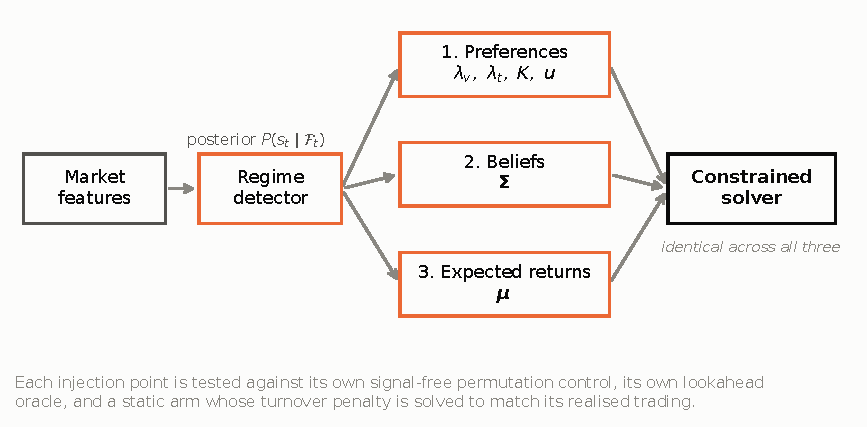
\includegraphics[width=\columnwidth]{figures/f12_injection_points.pdf}
\caption{The three points at which a detected state can act on a mean--variance
decision. All three feed one unchanged constrained solver, which is what makes them
comparable.}
\label{fig:injection}
\end{figure}

A three-state Gaussian HMM is fitted on realized volatility, a volatility ratio,
trailing return and drawdown, refit annually with a 36-month burn-in and a
two-month minimum dwell; states are ordered by fitted volatility into CALM,
TURBULENT and CRISIS. The detector uses \emph{filtered} posteriors
$P(s_t \mid \mathcal{F}_t)$ rather than smoothed posteriors --- a distinction
commonly lost in regime backtests that alone can manufacture the effect under test.

\textbf{Preferences.} The state selects risk aversion $\lambda_v$, turnover penalty
$\lambda_t$, cardinality $K$, position cap $u$ and two search parameters. This is
the analogue of regime-dependent risk aversion.

\textbf{Beliefs.} Each historical day $d$ is weighted by
$w_d = \sum_k P(s_t{=}k \mid \mathcal{F}_t) P(s_d{=}k \mid \mathcal{F}_d)$ and
$\boldsymbol{\Sigma}$ is the weighted second moment, shrunk toward a flat target.
In a crisis the risk model is built from past crisis days.

\textbf{Expected returns.} The state tilts $\boldsymbol{\mu}$ toward defensive
names, with strength posterior-weighted so a 55/45 call applies about half the
tilt. This is the only mechanism that relocates the optimum. We test tilts on a
transparent low-volatility score and on two \emph{exogenous} scores --- net share
issuance and market capitalization --- that the return panel cannot express.

%% =====================================================================
\section{Experimental Design}

\paragraph{Data and protocol.} CRSP daily securities, US common shares. The panel
spans 2005--2024; the evaluation window is 2011-01 to 2024-12, earlier years
reserved for standardization and burn-in. The universe is the 50 largest US common
stocks by market capitalization, reconstituted at each rebalance from information
available at that date, with delisting returns incorporated. Portfolios rebalance
monthly (168 decisions); targets computed at $t$ execute against $t$'s close, so a
decision never touches a return it also earns. Every arm runs at four cost levels
and 30 seeds, matched across arms. Causality is machine-checked: the panel is
poisoned after each decision date and the backtest re-run, asserting earlier
decisions are bit-identical and later ones are not.

\paragraph{Controls.} \emph{Permutation controls} permute the treatment's realized
label episodes, preserving state marginals and dwell-time distributions exactly
while destroying only timing. \emph{Lookahead oracles} fit the detector on the full
sample and reveal the labels; causally invalid by construction and reported as
upper bounds. \emph{No-timing parameterizations} hold the conditioned block fixed
throughout, separating having a parameterization from switching to it at the right
moment.

\paragraph{The turnover-matched control.} For each treatment we solve
\begin{equation}
\lambda_t^\star = \arg\min_{\lambda_t}
\bigl| \overline{\mathrm{TO}}(\text{static}; \lambda_t)
- \overline{\mathrm{TO}}(\text{treatment}) \bigr|
\end{equation}
by bisection. The calibration targets the treatment's \emph{turnover} --- a design
covariate read off its trading --- and never its Sharpe; calibrating on the outcome
would be circular. This is matching on a nuisance variable, as one matches a
control group on age. It is a control, not a deployable strategy.

\paragraph{Inference.} Arms are seed-matched, so we report paired differences.
Confidence intervals come from a stationary bootstrap~\cite{PolitisRomano1994} on
the paired daily difference series; Sharpe differences are additionally tested with
the HAC-robust statistic of~\citet{LedoitWolf2008}; families of comparisons receive
a Holm~\cite{Holm1979} correction.

\paragraph{Reproducibility.} Manifests record configuration, git SHA, package
versions, threading environment, and a content hash of the package source. The
source hash is necessary because a git SHA cannot identify the code that ran:
\texttt{git status} reports the whole tree, so regenerating a figure marks a run
dirty without a line of source changing, as it did for 450 of this study's first
719 runs. Reproduction is verified by re-execution, not asserted.

%% =====================================================================
\section{Results}

\subsection{Turnover orders everything}
\label{sec:ordering}

\begin{figure}[t]
\centering
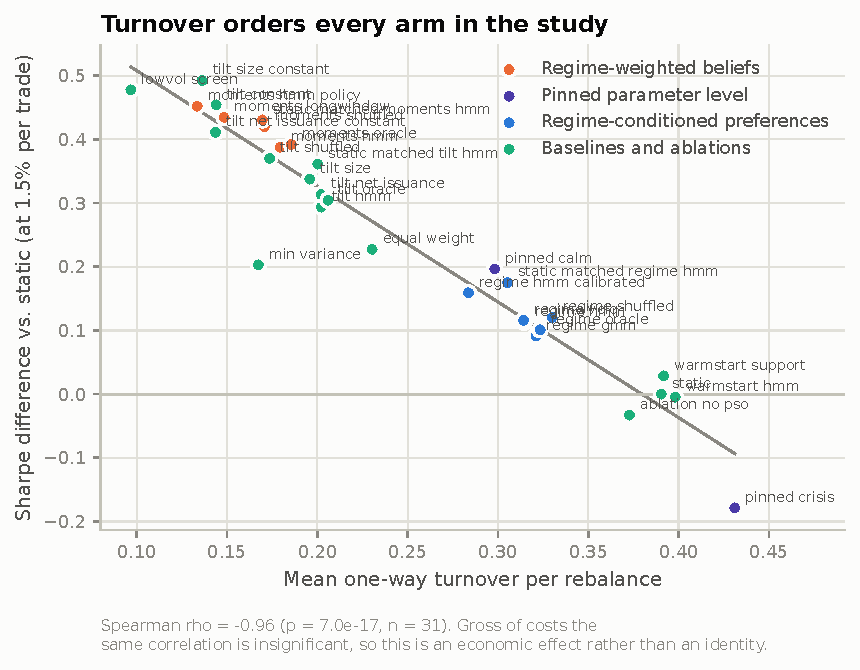
\includegraphics[width=\columnwidth]{figures/f8_turnover_explains_effect.pdf}
\caption{Net-of-cost Sharpe effect against realized turnover, one point per arm.
$\rho = -0.95$ ($p = 2.1\times10^{-14}$, $n = 27$); gross of costs the same
correlation is insignificant.}
\label{fig:turnover}
\end{figure}

\begin{table}[t]
\caption{Sharpe difference vs.\ \texttt{static} by transaction cost (per trade),
with mean one-way turnover. Abridged.}
\label{tab:arms}
\small
\begin{tabular}{lrrrr}
\toprule
Arm & 50 & 100 & 150 & TO \\
\midrule
\texttt{tilt\_constant} \emph{(no timing)}   & $+0.130$ & $+0.295$ & $+0.454$ & 0.144 \\
\texttt{moments\_longwindow} \emph{(no regime)} & $+0.117$ & $+0.278$ & $+0.435$ & 0.148 \\
\texttt{moments\_shuffled} \emph{(control)}  & $+0.132$ & $+0.278$ & $+0.420$ & 0.171 \\
\texttt{moments\_oracle} \emph{(lookahead)}  & $+0.124$ & $+0.261$ & $+0.392$ & 0.186 \\
\texttt{moments\_hmm} \emph{(treatment 2)}   & $+0.113$ & $+0.253$ & $+0.388$ & 0.179 \\
\texttt{tilt\_shuffled} \emph{(control)}     & $+0.097$ & $+0.236$ & $+0.370$ & 0.174 \\
\texttt{tilt\_oracle} \emph{(lookahead)}     & $+0.090$ & $+0.199$ & $+0.304$ & 0.206 \\
\texttt{tilt\_hmm} \emph{(treatment 3)}      & $+0.070$ & $+0.184$ & $+0.294$ & 0.202 \\
\texttt{equal\_weight}                       & $+0.024$ & $+0.128$ & $+0.227$ & 0.230 \\
\texttt{pinned\_calm} \emph{(no timing)}     & $+0.057$ & $+0.128$ & $+0.196$ & 0.298 \\
\texttt{regime\_shuffled} \emph{(control)}   & $+0.037$ & $+0.080$ & $+0.120$ & 0.330 \\
\texttt{regime\_hmm} \emph{(treatment 1)}    & $-0.002$ & $+0.057$ & $+0.113$ & 0.315 \\
\texttt{regime\_oracle} \emph{(lookahead)}   & $+0.006$ & $+0.055$ & $+0.101$ & 0.323 \\
\texttt{static}                              & $0$ & $0$ & $0$ & 0.390 \\
\texttt{ablation\_no\_pso}                   & $-0.028$ & $-0.031$ & $-0.033$ & 0.373 \\
\texttt{pinned\_crisis} \emph{(no timing)}   & $-0.079$ & $-0.131$ & $-0.179$ & 0.431 \\
\bottomrule
\end{tabular}
\end{table}

Table~\ref{tab:arms} orders arms by their effect at 150\,bps. Read by the final
column instead and the ranking reproduces almost exactly. Across the 27 comparable
arms the rank correlation between realized turnover and the net-of-cost effect is
$\rho = -0.95$ ($p = 2.1\times10^{-14}$); gross of costs it is $\rho = +0.25$
($p = 0.21$). The ordering is an economic effect operating through realized trading
costs, not an accounting identity.

Three readings follow. \textbf{A control beats its treatment:}
\texttt{regime\_shuffled} gains $+0.120$ against the treatment's $+0.113$, and
\texttt{tilt\_shuffled} $+0.370$ against $+0.294$. \textbf{The absence of timing
beats timing:} \texttt{pinned\_calm}, which never switches, gains $+0.196$ ---
nearly double \texttt{regime\_hmm}. \textbf{Perfect future knowledge buys nothing:}
every oracle sits at or below a regime-free arm in its family. Gross of costs, the
five best arms are all unconditional; every mechanism examined gives up gross
return and earns its net advantage by trading less.

\subsection{The turnover-matched control}
\label{sec:matched}

\begin{figure}[t]
\centering
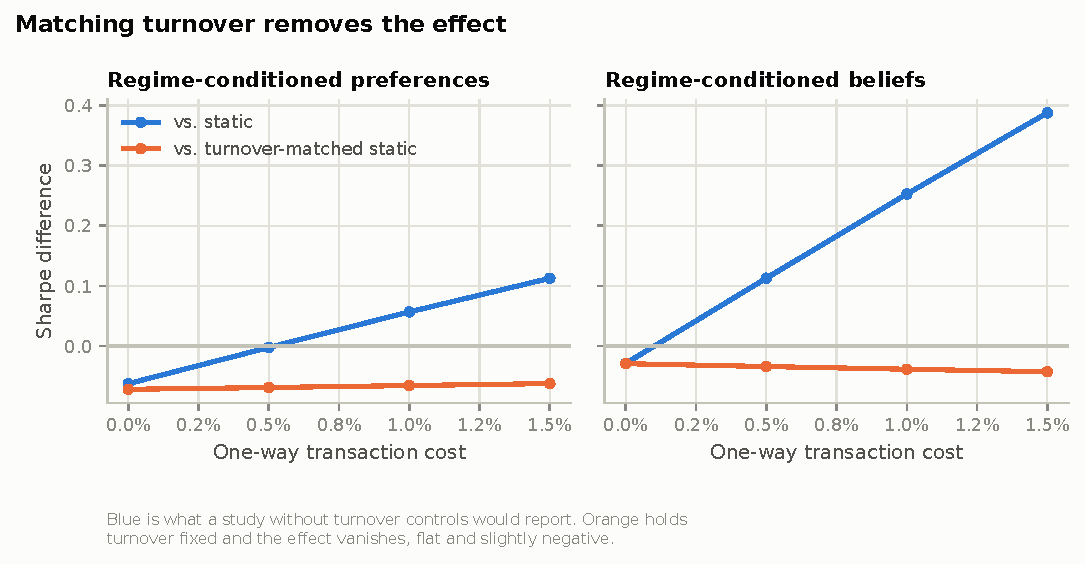
\includegraphics[width=\columnwidth]{figures/f9_turnover_matched.pdf}
\caption{Each mechanism's effect across the cost sweep against an unmatched
baseline (rising steeply) and a turnover-matched control (flat, slightly negative).}
\label{fig:matched}
\end{figure}

\begin{table}[t]
\caption{Regime effect against a turnover-matched control.}
\label{tab:matched}
\small
\begin{tabular}{lrrr}
\toprule
Injection point & TO (t/c) & @50\,bps & @150\,bps \\
\midrule
Preferences      & 0.315/0.305 & $-0.069$ & $-0.062$ \\
Beliefs          & 0.179/0.170 & $-0.034$ & $-0.043$ \\
Expected returns & 0.202/0.200 & $-0.047$ & $-0.067$ \\
\bottomrule
\end{tabular}
\end{table}

The regime signal does not merely stop helping once turnover is held fixed --- it
is consistently negative, at every injection point and every cost level. Only
mechanism 1's effect is individually significant (Ledoit--Wolf $p = 0.039$ at
50\,bps); the others sit well inside noise, which is itself informative given
Section~\ref{sec:noise}.

\textbf{The strongest evidence is the shape, not the level.} Measured against the
unconditional baseline the three effects swing by $+0.176$, $+0.417$ and $+0.340$
across the cost sweep, each flipping from negative to positive as costs rise ---
exactly the signature that makes conditioning look valuable to a cost-aware
investor. Measured against the matched control those swings collapse to
approximately zero and turn slightly negative. That is what ``turnover was the
mechanism'' predicts, and no competing explanation predicts it.

\subsection{Why each mechanism fails}

\ICAIFcut
\textbf{Preferences modulate over stale beliefs.} Half the conditioned parameters
govern how the search proceeds rather than what it optimizes; the rest change the
objective but act on moments estimated from a flat 252-day window that is itself
regime-blind. In March 2020 the mechanism tells the optimizer to fear risk while
handing it a covariance matrix dominated by the preceding eleven calm months.

\textbf{Beliefs are confounded with window length.} \texttt{moments\_hmm} gains
$+0.388$ at 150\,bps, but \texttt{moments\_longwindow} --- the same five-year
lookback with \emph{no regime weighting} --- gains $+0.435$. The regime-weighted
estimator requires a long window because weighting discards non-matching days, and
that window is itself stabilizing. Without this control the study would have
reported a large, entirely spurious effect.

\textbf{Expected-return tilts fail hardest.} The mechanism with the strongest prior
claim is the most decisively null: \texttt{tilt\_hmm} is the worst arm in its own
family, below its shuffled control, below every no-timing constant, below its
turnover-matched control, and $+0.010$ below its own oracle. Tilts on exogenous
scores the return panel cannot express behave identically, so the failure is not an
artifact of deriving the signal from the same returns that produce the moments.

\textbf{Detector quality is not binding.} A transparent rule (volatility terciles,
nothing fitted) matches the fitted HMM at every cost level.

\subsection{The noise floor}
\label{sec:noise}

\begin{figure}[t]
\centering
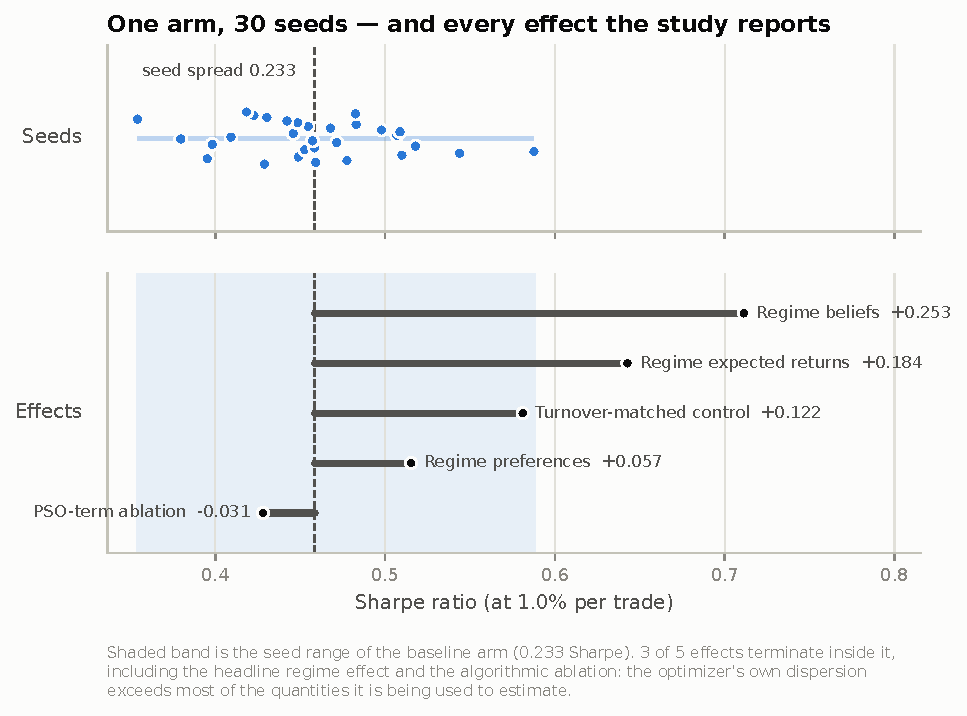
\includegraphics[width=\columnwidth]{figures/f10_noise_floor.pdf}
\caption{The study's effect sizes drawn inside the seed spread of its own baseline
arm at 100\,bps per trade.}
\label{fig:noise}
\end{figure}

Re-running the unconditional arm with a different seed changes nothing about the
data, configuration or universe. It changes the answer. At 100\,bps the 30 seeds
span Sharpe $0.354$--$0.588$ (spread $0.233$, SD $0.049$) and fourteen-year
terminal wealth $1.98\times$--$3.66\times$, a ratio of $1.85\times$. Against the
effects measured at that cost --- beliefs $+0.253$, expected returns $+0.184$, the
matched comparison $+0.122$, preferences $+0.057$, the ablation $-0.031$ ---
\textbf{three of five fall inside the seed range}, including the headline regime
effect.

This does not overturn Sections~\ref{sec:ordering}--\ref{sec:matched}: with 30
seeds the standard error of the mean paired difference is $0.012$--$0.015$, so
effects with $|t| > 3$ stand. \textbf{The study is saved by its sample size}, and a
comparable single-seed study --- as most in this literature are --- would be
reporting noise.

A restart probe at six dates, sweeping the blend across pure firefly, the hybrid,
and pure PSO, finds a \emph{typical} run falls 26--45\% short of a reference budget
for all three. The stronger claim that no amount of restarting closes the gap does
\emph{not} hold: pure firefly's best-of-60 restarts beat the reference at two of
six dates. The claim belongs at the typical-run level, which is the level at which
this literature reports.

\subsection{What the optimizer can defend}
\label{sec:conviction}

\begin{figure}[t]
\centering
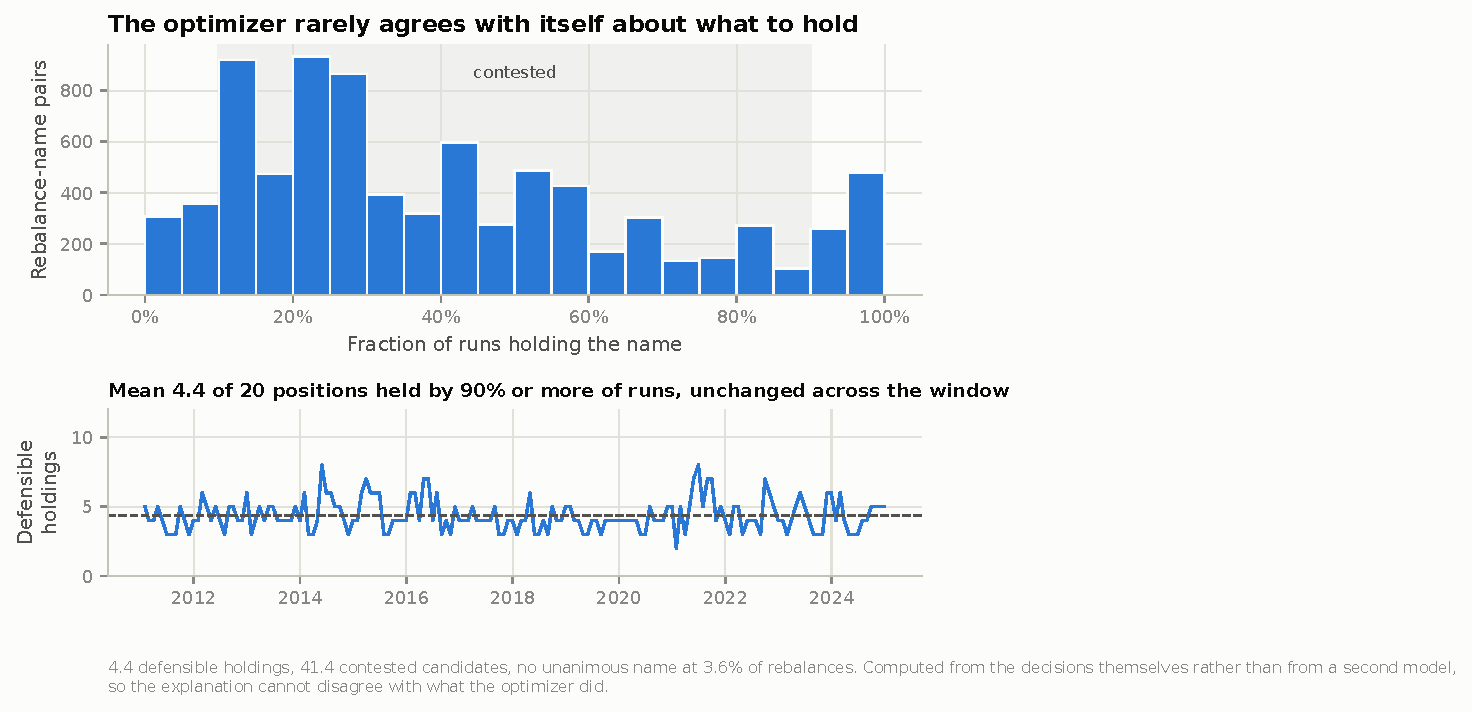
\includegraphics[width=\columnwidth]{figures/f11_conviction.pdf}
\caption{Cross-run inclusion frequency, and the count of defensible holdings over
time.}
\label{fig:conviction}
\end{figure}

At every one of the 168 rebalances the 30 seeds produce 30 distinct supports; no
two ever select the same 20 names. The fraction of runs holding an asset is
computed from the decisions themselves rather than generated by a second model, so
unlike a post-hoc attribution it cannot disagree with what the optimizer did.

Of the 20 positions held, \textbf{4.4 on average appear in 90\% or more of runs}.
Around 41 of roughly 49 candidates are contested, and 3.6\% of rebalances produce
no unanimous name. \textbf{And it does not move}: the annual mean ranges
$3.83$--$5.17$ across fourteen years and roughly seven crisis episodes. Decision
ambiguity here is a property of the search, not of market conditions --- a second,
independent corroboration of Section~\ref{sec:noise}.

\begin{table}[t]
\caption{PSO-term ablation at 30 and 52 matched seeds.}
\label{tab:ablation}
\small
\begin{tabular}{llrrrr}
\toprule
Seeds & Cost & Effect & SE & $t$ & Boot.\ $p$ \\
\midrule
30 & 50\,bps  & $-0.032$ & 0.013 & $-2.48$ & 0.336 \\
30 & 150\,bps & $-0.034$ & 0.016 & $-2.22$ & 0.271 \\
52 & 50\,bps  & $-0.028$ & 0.009 & $\mathbf{-3.03}$ & 0.391 \\
52 & 150\,bps & $-0.031$ & 0.011 & $\mathbf{-2.77}$ & 0.307 \\
\bottomrule
\end{tabular}
\end{table}

\textbf{The ablation, and a limit on what compute can buy.} Removing the PSO term
costs $-0.03$ Sharpe, consistent in sign at every cost level. A seed-level power
analysis prescribed 52 seeds, so we ran both arms at 52
(Table~\ref{tab:ablation}). The extra seeds did what the analysis predicted along
the seed dimension --- the estimate is stable, the cross-seed standard error falls
by a third, and the per-seed $t$ crosses 3 --- and did \emph{not} move the
time-series inference at all. The per-seed statistic treats paired differences as
independent draws and shrinks without limit; the bootstrap operates on the
seed-averaged daily path and is bounded by fourteen years of history, which
computation does not extend. \textbf{Seed replication buys precision about the
optimizer, not statistical power about the market.} We report the effect as real in
sign, stable in magnitude, and unresolvable in this sample.

%% =====================================================================
\section{Discussion}

\ICAIFcut
\paragraph{Three confounds the controls caught.} Each produced plausible numbers
and broke no test. \emph{(i)} The falsification control silently degenerated: it
originally sampled labels from the fitted transition matrix, and because the chain
is persistent only for CALM, the minimum-dwell smoother filtered stressed episodes
away. The control collapsed to 97\% CALM and, because CALM is the low-turnover
configuration, \emph{looked like the best arm in the study}. \emph{(ii)}
Mechanism~2's effect was a window-length artifact, caught by adding
\texttt{moments\_longwindow}. \emph{(iii)} A determinism guarantee was passing for
the wrong reason: multithreaded BLAS made the detector posterior differ at
$\sim\!10^{-14}$ between runs, which arms taking $\arg\max$ absorbed and arms
weighting continuously by the posterior did not. Seven of 32 arms were not
bit-reproducible, and the split across the matrix was exact. The magnitude changed
no conclusion; the lesson does not depend on it. \textbf{When a mechanism changes
more than one thing, every changed thing needs its own control arm.}

\paragraph{Interpretation.} Turnover reduction is a real economic benefit, but it
is available directly, more cheaply and more controllably through a turnover
penalty --- without fitting a hidden Markov model, without its estimation risk, and
without the implicit claim that the strategy knows something about the market's
state. The recommendation follows: \emph{if a conditional allocation strategy is
reported to beat an unconditional baseline net of costs, the comparison that
matters is against a turnover-matched control.}

\paragraph{Limitations.} One universe, one objective, one metaheuristic, one asset
class, and a window containing roughly seven crisis episodes. The restart probe
sweeps a blend within one algorithm family; all three configurations share a repair
operator and are three points on one axis rather than three independent algorithms.
Our positioning also rests on a claim about absence --- that this literature does
not report turnover-matched controls --- which we state for the works cited in
Section~2 on the basis of their reported results tables, and not of the literature
as a whole. We do not establish that regime conditioning cannot work; we establish
that here, at three natural injection points, the measured effect was turnover, and
that a control capable of detecting this was necessary to find out.

%% =====================================================================
\section{Conclusion}

We injected a market-regime signal at each of the three points where it can act on
a constrained mean--variance decision, and measured each against a permutation
control, a lookahead oracle, and an unconditional arm solved to trade exactly as
much as the treatment. Measured the way this literature measures, all three
mechanisms work. None survives control. \textbf{In this setting, regime effects in
constrained portfolio optimization are turnover effects.}

We also quantified the noise floor of the instrument that produced these numbers:
re-running one arm under a different seed moves realized Sharpe by $0.233$ and
terminal wealth by $1.85\times$, exceeding three of the five effects reported here.
The study survives that only because it runs 30 seeds; most of this literature runs
one. We release the harness, because it caught three silent confounds in this study
and because the protocol generalizes well beyond the mechanism we used it to test.

\bibliographystyle{ACM-Reference-Format}
\bibliography{refs}

\end{document}
